\documentclass[11pt]{article}
\usepackage[margin=1in]{geometry}
\usepackage{amsmath,amssymb,amsthm,graphicx,microtype}
\usepackage[hidelinks]{hyperref}
\emergencystretch=3em

\newtheorem{theorem}{Theorem}
\newtheorem{remark}[theorem]{Remark}
\newcommand{\Ran}{\operatorname{Ran}}
\newcommand{\cN}{\mathbb N}

\title{A Full Affirmative Answer to the\ Fractional-Range Question for Cyclic Projections}
\author{Literature-implied answer packet for arXiv:1510.04560\\
\texttt{fa\_banach\_001}, lane 8, \texttt{agent\_lane\_08}}
\date{11 August 2026}

\begin{document}
\maketitle

\begin{center}
\fbox{\parbox{0.91\textwidth}{
\textbf{Status: literature-implied answer (full).}
For every finite family of closed subspaces and every $0<\alpha<1/2$,
the algebraic sum of their orthogonal complements is contained in
$\Ran(I-T)^\alpha$.  Thus the question in Badea--Seifert has a full
affirmative answer, with a uniform interval of exponents and without the
aligned-case hypothesis.  The proof combines Reich--Zalas's later operator
estimate with the binomial functional calculus.  This implication appears
not to have been stated in the supporting paper and is identified here.
}}
\end{center}

\section{Source question}

Let $M_1,\ldots,M_N$ be closed subspaces of a real or complex Hilbert space
$X$, let $P_i=P_{M_i}$, and set
\[
 T=P_N\cdots P_1.
\]
Badea and Seifert \cite[Remark 4.4(b), PDF p.~14]{BS} ask, in the aligned
case, whether
\begin{equation}\label{eq:source}
 M_1^\perp+\cdots+M_N^\perp\subseteq\Ran(I-T)^\alpha
\end{equation}
for some $\alpha\in(0,1)$, or at least whether the left-hand side is
contained in $\bigcup_{\alpha>0}\Ran(I-T)^\alpha$.  They note that either
inclusion would imply a conjecture of Deutsch and Hundal concerning the
location of vectors witnessing arbitrarily slow cyclic-projection
convergence.

\begin{figure}[p]
\centering
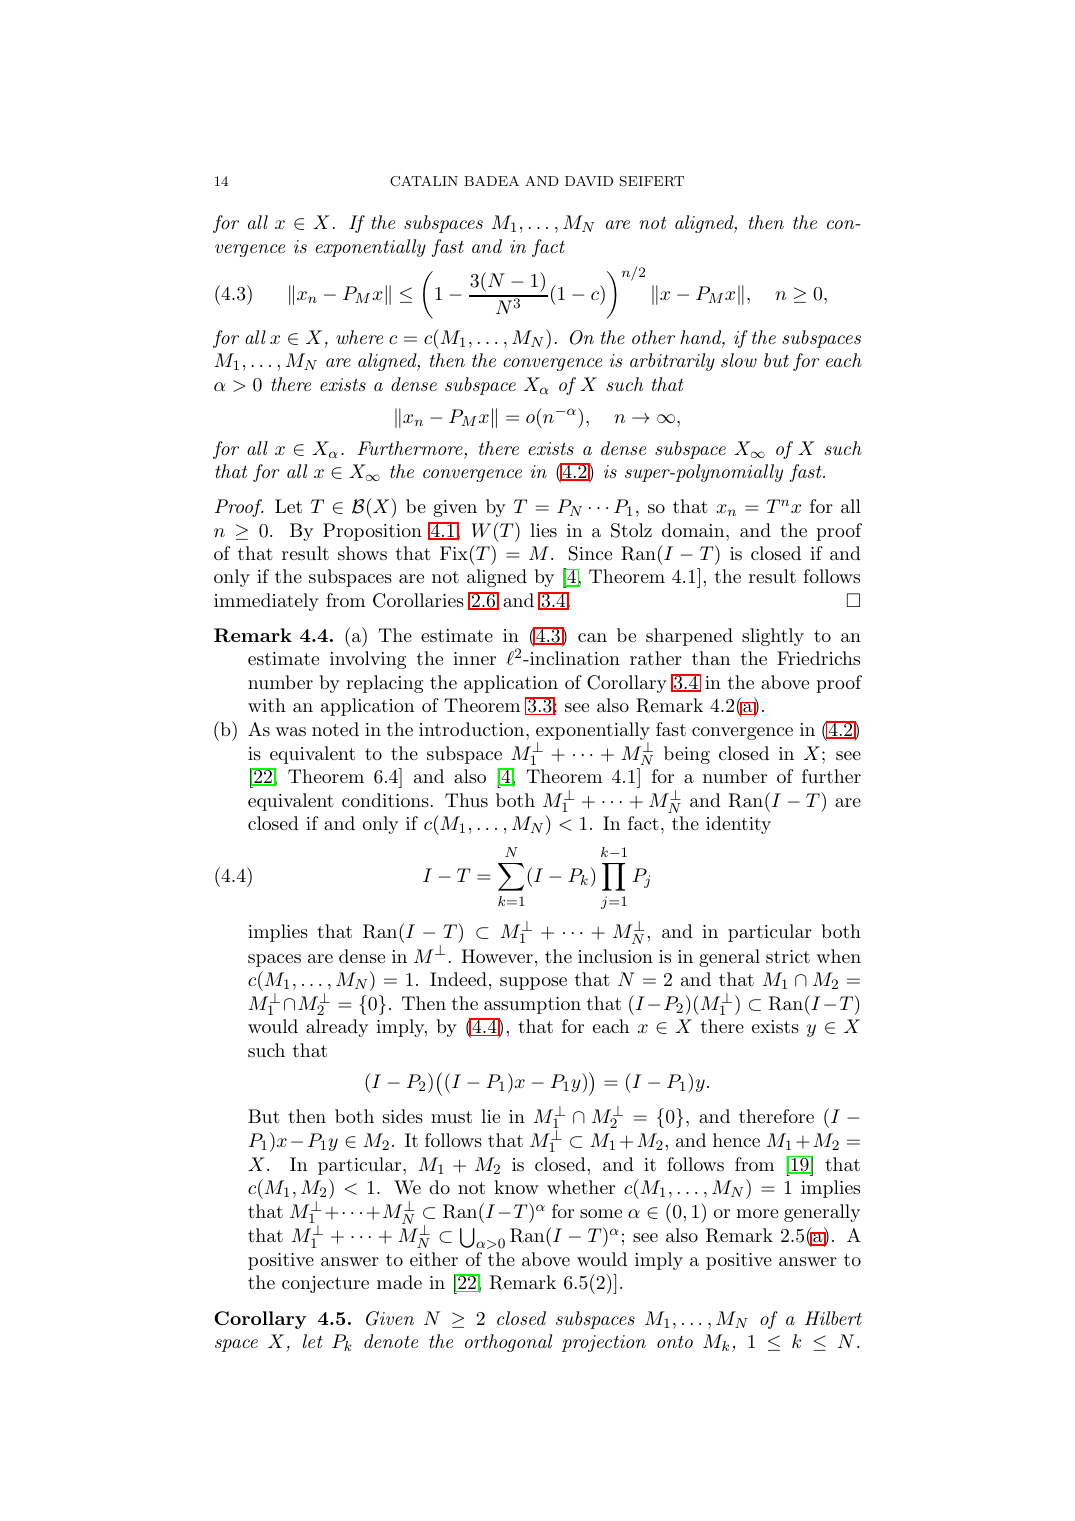
\includegraphics[width=0.96\textwidth,height=0.82\textheight,keepaspectratio]{figures/source_question_page14.png}
\caption{Badea--Seifert, arXiv:1510.04560, PDF page 14.  The fractional-range
question appears near the bottom of Remark 4.4(b).}
\end{figure}
\clearpage

\section{Later estimate and the answer}

Write $Q_i=P_{M_i^\perp}=I-P_i$.  Reich and Zalas prove the following
operator-norm estimate \cite[Lemma 4.1(iii), PDF p.~10]{RZ}:
\begin{equation}\label{eq:RZ}
 \max_{1\le i\le N}\|T^nQ_i\|=O(n^{-1/2}).
\end{equation}
Their paper is written for real Hilbert spaces.  For a complex Hilbert space,
apply the estimate to its underlying real Hilbert space; the projections,
products, and operator norms are unchanged.

\begin{theorem}\label{thm:main}
For arbitrary closed subspaces $M_1,\ldots,M_N$ of a real or complex Hilbert
space and $T=P_N\cdots P_1$, one has
\[
 M_1^\perp+\cdots+M_N^\perp\subseteq\Ran(I-T)^\alpha
 \qquad\text{for every }0<\alpha<\tfrac12.
\]
More precisely, for each $i$ there is a bounded operator $B_i$ such that
\begin{equation}\label{eq:factor}
 (I-T)^\alpha B_i=Q_i.
\end{equation}
\end{theorem}

\begin{proof}
Fix $0<\alpha<1/2$.  Let
\[
 c_n=\frac{\Gamma(n+\alpha)}{\Gamma(\alpha)\Gamma(n+1)},
 \qquad n\ge0,
\]
so that $(1-z)^{-\alpha}=\sum_{n\ge0}c_nz^n$ for $|z|<1$ and
$c_n=O((n+1)^{\alpha-1})$.  For each $i$, define
\begin{equation}\label{eq:Bi}
 B_i=\sum_{n=0}^\infty c_nT^nQ_i.
\end{equation}
By \eqref{eq:RZ}, this series converges absolutely in operator norm, since
\[
 \sum_{n=0}^\infty c_n\|T^nQ_i\|
 \ \lesssim\ 1+\sum_{n=1}^\infty n^{\alpha-3/2}<\infty.
\]

On the other hand, the standard binomial functional calculus for the
contraction $T$ gives the absolutely convergent series
\begin{equation}\label{eq:positive}
 (I-T)^\alpha=\sum_{m=0}^\infty d_mT^m,
 \qquad d_m=(-1)^m\binom{\alpha}{m}.
\end{equation}
Indeed, $|d_m|=O(m^{-\alpha-1})$.  The product of \eqref{eq:Bi} and
\eqref{eq:positive} is an absolutely convergent double series: because $T$
is a contraction,
\[
 \sum_{m,n\ge0}|d_m|c_n\|T^{m+n}Q_i\|
 \leq \left(\sum_{m\ge0}|d_m|\right)
       \left(\sum_{n\ge0}c_n\|T^nQ_i\|\right)<\infty.
\]
We may therefore take its Cauchy product.  The scalar generating functions
satisfy $(1-z)^\alpha(1-z)^{-\alpha}=1$, and hence
\[
 (I-T)^\alpha B_i
 =\sum_{k=0}^\infty
   \left(\sum_{m+n=k}d_mc_n\right)T^kQ_i
 =Q_i.
\]
This proves \eqref{eq:factor}.  Finally, if
$x=x_1+\cdots+x_N$ with $x_i\in M_i^\perp$, then
\[
 x=\sum_{i=1}^NQ_ix_i
   =(I-T)^\alpha\left(\sum_{i=1}^NB_ix_i\right),
\]
which proves the asserted range inclusion.
\end{proof}

\begin{figure}[p]
\centering
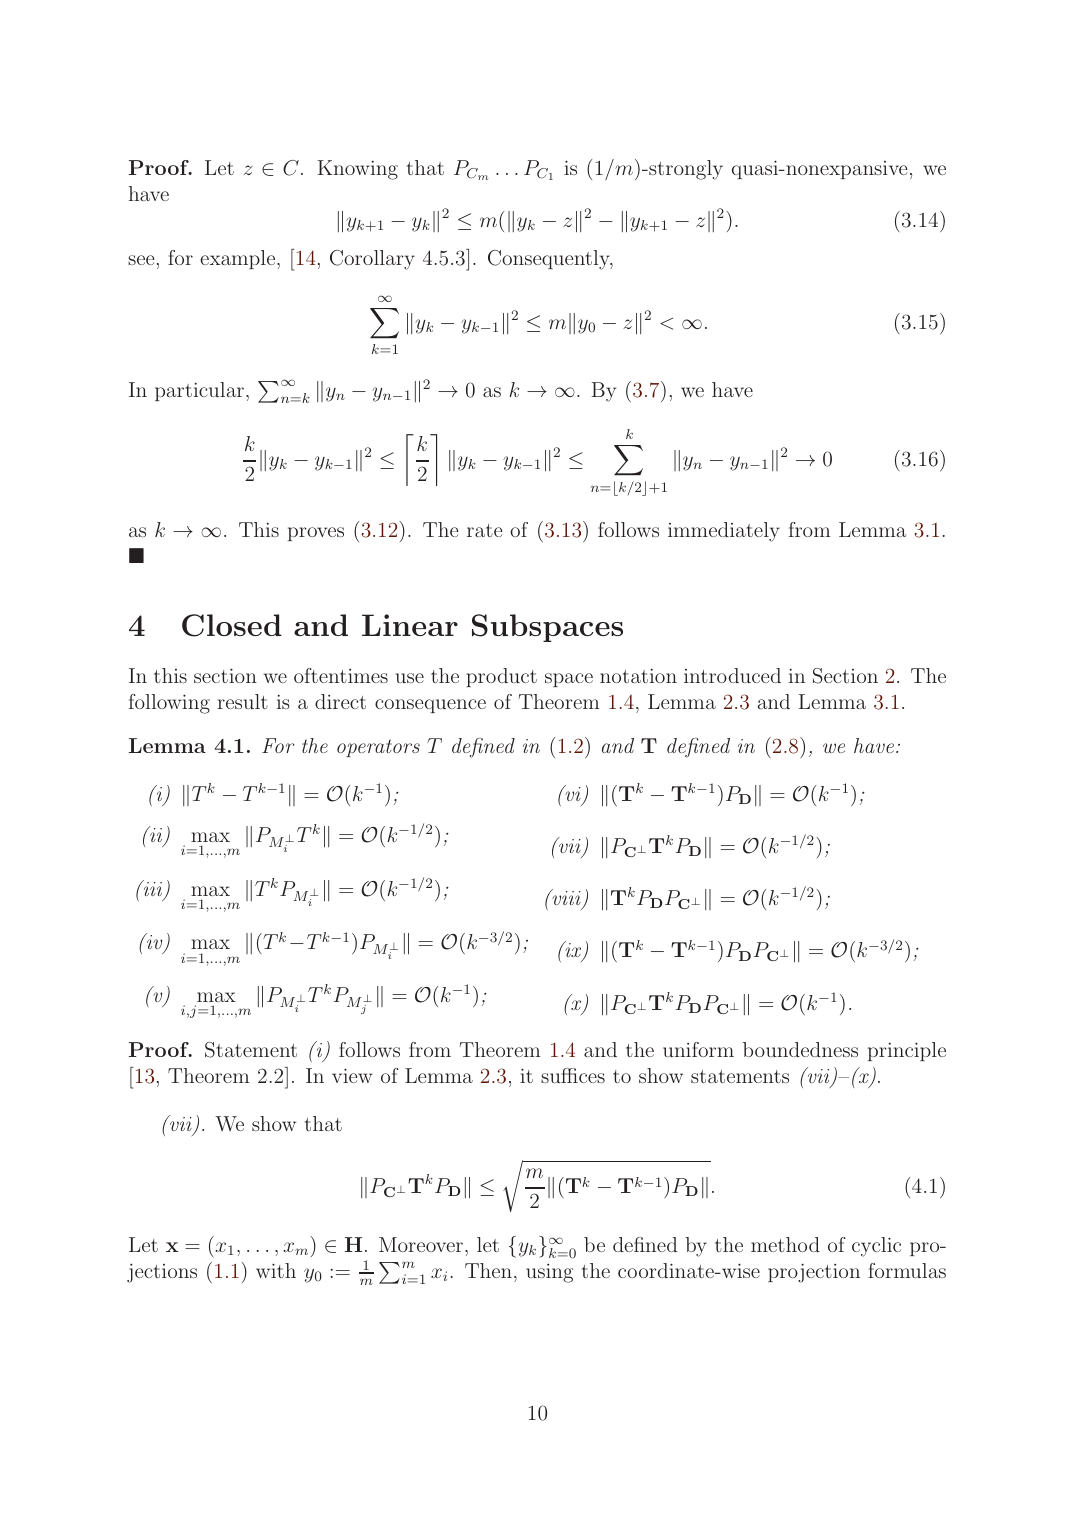
\includegraphics[width=0.96\textwidth,height=0.82\textheight,keepaspectratio]{figures/reich_zalas_lemma_page10.png}
\caption{Reich--Zalas, arXiv:2205.13843, PDF page 10.  Lemma 4.1(iii) is the
operator estimate used in the factorization.}
\end{figure}
\clearpage

\section{Consequences, scope, and provenance}

The theorem answers the stronger first alternative in the source question.
It also gives more than was requested: the inclusion holds for every
$\alpha\in(0,1/2)$, and no alignment assumption is needed.  In particular,
every vector in
$M\oplus(M_1^\perp+\cdots+M_N^\perp)$, where
$M=\bigcap_iM_i$, has at least the polynomial convergence supplied by the
fractional-power theory.  Reich and Zalas directly prove the sharper orbit
bound $O(n^{-1/2})$ on this subspace in their Theorem 4.3.

The strict inequality $\alpha<1/2$ is exactly what makes the norm series
\eqref{eq:Bi} summable from the known $n^{-1/2}$ estimate.  The argument does
not settle the endpoint $\alpha=1/2$, but the source question only asks for
one exponent in $(0,1)$.

A bounded search using the arXiv identifiers, titles, exact range notation,
and the core cyclic-projection keywords located no paper explicitly stating
this factorization or the resulting answer to Remark 4.4(b).  The supporting
paper proves \eqref{eq:RZ} and the orbit-rate consequences, not the
fractional-range inclusion.  Accordingly, this packet is classified as a
\emph{literature-implied} full answer and makes no claim that Reich and Zalas
presented it as an answer to Badea--Seifert.

\begingroup\raggedright
\begin{thebibliography}{9}
\bibitem{BS}
C. Badea and D. Seifert,
\emph{Ritt operators and convergence in the method of alternating
projections}, J. Approx. Theory 205 (2016), 133--148;
arXiv:1510.04560.

\bibitem{RZ}
S. Reich and R. Zalas,
\emph{Polynomial estimates for the method of cyclic projections in Hilbert
spaces}, Numer. Algorithms 94 (2023), 1217--1242;
arXiv:2205.13843, doi:10.1007/s11075-023-01533-w.
\end{thebibliography}
\endgroup

\end{document}
